\documentclass[a4paper,12pt]{article}
%\documentclass[a4paper,10pt]{scrartcl}

\usepackage[margin=0.8in]{geometry}
\usepackage[utf8]{inputenc}
\usepackage{graphicx}
%\documentclass{minimal}
\usepackage{amsmath}
\usepackage{xcolor}
\usepackage{listings}
\lstset{
    frame=single,
    breaklines=true,
    postbreak=\raisebox{0ex}[0ex][0ex]{\ensuremath{\color{red}\hookrightarrow\space}}
}
\lstdefinelanguage{numpy}{
    keywords = {mean}
}

\title{Synchronization of Lines in an Image}
\author{B098688}
\date{\today}



\begin{document}
\maketitle

\begin{abstract}
 This report outlines a proposed procedure for synchronising lines of an image that has been corrupted by randomly shifting horizontal lines. The method involves the use of Discrete Fourier Transforms of each line in the given image to determine to what degree each of them was shifted. The end result of the procedure is an image that has been reconstructed to an almost perfect extent, with the edges of the output images being the most notorious unfixed problem.
\end{abstract}

\section{Introduction}

The field of digital image processing aims to modify images through the use of various mathematical operations. This is done by considering images as two dimensional objects and applying signal processing techniques to them in order to manipulate them~\cite{gonzalez1992digital}. This work describes an algorithm that uses image processing techniques to synchronise an image. In this particular case, said input image has had certain horizontal lines randomly shifted. The input corrupted image must be in file format \texttt{.pgm} (Portable Graymap), since this file format can be read as a two dimensional array, for example fig.~\ref{fig.1}. After passing the input image through the devised algorithm, the output should have most lines shifted into their appropriate location. Some information is lost in the output image - this occurs mainly in the image's edges, this will be elaborated in the next section.

\begin{figure}[h!]
\centering
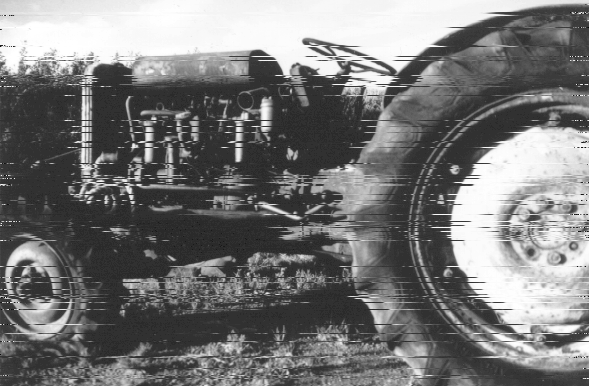
\includegraphics[width=0.73\textwidth]{img/desync2}
\caption{Randomly shifted horizontal lines.}
\label{fig.1}
\end{figure}

The algorithm used to attempt to synchronise the horizontal lines of the given images was written in Python3.5, and imports the libraries: \texttt{os} for handling the input and output of images (hopefully) without errors, \texttt{matplotlib.pyplot} for showing the enhanced image (which is then optionally saved by the user), \texttt{misc} from \texttt{scipy} to read the \texttt{.pgm} input files and write the output file, and \texttt{numpy} since it allows for the use of Discrete Fourier Transform (DFT, which are a fundamental component of the algorithm). Version control was implemented in the development of the algorithm. Consequently, the code is available in a public \texttt{github} repository under the following url: \texttt{https://github.com/quietF/NumRep} on the folder \texttt{FT}. There, a short \texttt{README} file details the implementation of the code. Nevertheless, the code is also included in an annex in the end of this report. 

In broad terms, which will be elaborated on later on, the algorithm takes the two dimensional image and compares vertically adjacent lines by calculating the cross correlation between them. From this, the number of pixels that these lines have been shifted is obtained. This allows for a reconstruction of the image. Some limiting cases must be considered to get the enhanced image. It must be said that the developed algorithm can be improved since not all images are perfectly reconstructed. The following sections will elaborate on this. 

\section{Aim and Methods}

The aim of this problem is to take an image in grayscale format with an arbitrary number of horizontally shifted lines and attempt to place them in their right position. Since the line desynchronisation is exclusive to the horizontal direction, i.e. no lines have a vertical shift, it is sensible to divide the two dimensional image into a series of one dimensional objects, where each object is a horizontal line. 

Through the use of various mathematical methods it is possible to find the degree to which each horizontal line has been shifted. The method described, and used, relies on a very strong assumption - vertically adjacent lines can be considered as being approximately equal. This is justified by the fact that most lines in the input images will indeed be very similar. For example, lines \#0 and \#1 from one of the images are plotted as a signal in fig.~\ref{fig.2} and~\ref{fig.3}. This, however, will not always be true, and will lead to problems in the algorithm. Since the one dimensional objects, horizontal lines, are being treated as signals, it is adequate to look for signal processing tools to find how to synchronise the lines. An operation that compares two signals for their similarity is necessary. This is precisely the cross correlation of two functions.

\begin{figure}[h]
\centering
\begin{minipage}{.5\textwidth}
  \centering
  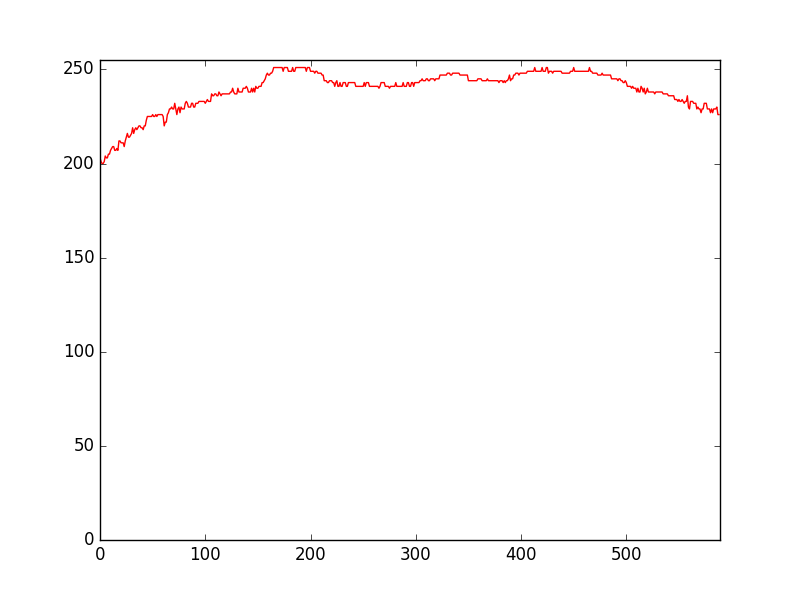
\includegraphics[width=1.05\linewidth]{img/line0}
  \caption{Horizontal line \#0 from the top.}
  \label{fig.2}
\end{minipage}%
\begin{minipage}{.5\textwidth}
  \centering
  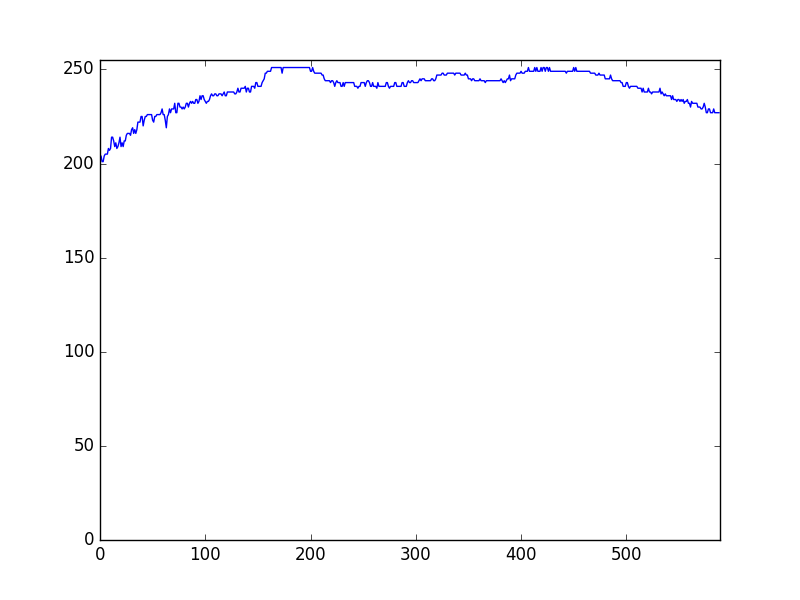
\includegraphics[width=1.05\linewidth]{img/line1}
  \caption{Horizontal line \#1 from the top.}
  \label{fig.3}
\end{minipage}
\end{figure}

If two signals are defined by functions $f(t)$ and $g(t)$, then the cross correlation between the two signals is defined as eqn.~\ref{eq.1}, where the notation for complex conjugate is $f^*$, as usual~\cite{bracewell2012fourier}.  

\begin{equation}
 (f \star g)(\tau) = \int_{-\infty}^{\infty} f^*(t) g(t+\tau) dt
 \label{eq.1}
\end{equation}

This can be expressed in a much more simple fashion, by making use of the properties of the Fourier Transforms. Doing so results in a much more simple expression for the cross correlation between two signals. This expression is shown in eqn.~\ref{eq.2}, where $\mathcal{F}\{ f \}$ denotes the Fourier Transform of the signal $f$~\cite{bracewell2012fourier}.

\begin{equation}
 \mathcal{F}\{ f \star g \}(\tau) = (\mathcal{F}\{ f \})^* \cdot \mathcal{F}\{ g \}
 \label{eq.2}
\end{equation}

This means that if the Fourier Transform of each line can be obtained, then retrieving the cross correlation between lines is simply a multiplication, followed by an Inverse Fourier Transform. Luckily, the scientific computing package available for Python, \texttt{numpy}, has a simple way of obtaining the Discrete Fourier Transform (DFT) of an array (as well as its Inverse DFT). These are all methods under the routine \texttt{numpy.fft} (which stands for ``fast Fourier Transform''). Figure~\ref{fig.4} shows exactly this by taking the normalised cross correlation of both signals in fig.~\ref{fig.2} and~\ref{fig.3}. 

\begin{figure}[h!]
\centering
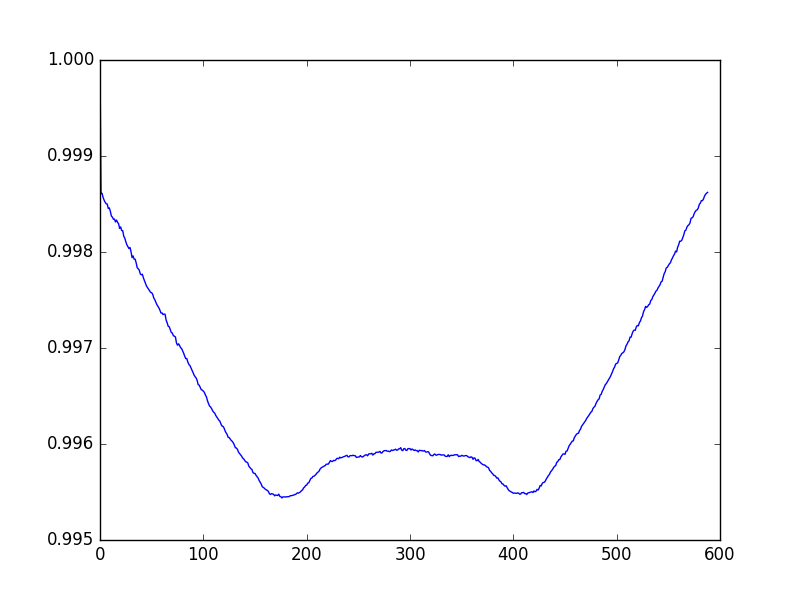
\includegraphics[width=0.8\textwidth]{img/xcorrelation}
\caption{Cross correlation of fig.~\ref{fig.2} and~\ref{fig.3}.}
\label{fig.4}
\end{figure}

The maximum of the cross correlation is located at 0 in the x axis. This means that no shift needs to be made in order to maintain the two images as the ``same''. When this maximum is not located at 0, then it is likely that a shift needs to be made in order to synchronise those lines. From this a basic idea of what the algorithm has to be can be devised. The process would be something along these lines: 

\begin{enumerate}
 \item Obtain the DFT of line \#i and of line \#i-1.
 \item Obtain the normalised cross correlation of the two DFTs.
 \item Shift line\#i such that the cross correlation maximum is located at 0.
\end{enumerate}

Following said method for all lines (excluding line \#0 as it has no line above to compare) should reconstruct the image to its right position. The result for fig.~\ref{fig.1} after going through the method described is shown in fig.~\ref{fig.5}. Clearly something has gone wrong and the shift has been too careless, but not everything is bad. Other than the edges, the image has been reconstructed to an acceptable extent. However, this can be improved.

\begin{figure}[h!]
\centering
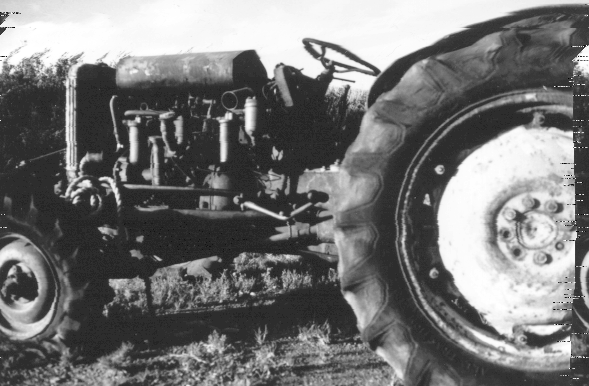
\includegraphics[width=0.73\textwidth]{img/simple}
\caption{First synchronising method for fig.~\ref{fig.1}.}
\label{fig.5}
\end{figure}

As it can be seen in the image above, on the right hand side, it looks like the image had a horizontal shift that was not meant to occur and the rest of lines followed from it - such behaviour will be called ``bulk'' shifting. This lead to believing that there must be some sort of threshold that attempts catching lines that have the cross correlation maximum located somewhere different than zero, but should not be shifted. 

After observing ``bulk'' shifting in other test images, a condition was made in order to prevent it. It basically requires that two consecutive shifts are not made by the same number of pixels. This can be reconciled with the fact that the input image has horizontal shifts by some random number of pixels, and it would be unlikely that two consecutive lines were randomly shifted by the same number of pixels. 

Nevertheless, the ``bulk'' shifting solution would only fix the problem of consecutive lines being shifted, and not the problem with shifting lines that should not have been shifted in the first place. To avoid this problem, a lower and a higher bound for the maximum value of the cross correlation is used when considering whether or not to shift a line. 

This ends up with the following method:

\begin{enumerate}
 \item Obtain the DFT of line \#i and of line \#i-1.
 \item Obtain the normalised cross correlation of the two DFTs.
 \item Check that the shift of line \#i-1 is different from that of line \#i.
 \item Check that the maximum value of the cross correlation is within appropriate bounds.
 \item Conditionally shift line \#i. 
\end{enumerate}

This method provides successful results, which seem to be better for larger images with more detail, but is not able to fix ``scratchy'' edges.

\section{Results}

As a short recap, the developed algorithm takes an input image with an arbitrary number of horizontal lines shifted randomly, with the idea of synchronising the image's lines. This is done by separating the two dimensional image into a series of lines - which are then considered as signals. Through the use of signal processing comparison methods it is possible to find the number of pixels each horizontal line was shifted. Using this and applying other, more empirical, approaches it was possible to obtain a good set of output images. 

For the first image - that of some medieval building - the reconstruction is not entirely great. A few lines were not shifted by the algorithm and there is some information lost on the edges. Whether or not an algorithm can be devised such that the output image is perfect is not clear. This would require that the horizontal shifts were performed in a periodic manner, as \texttt{numpy} does the array shifting in a periodic manner. It appears that this is not the case, and to remove the ``scratchy'' edges some method to copy the line above (or a section of it) could be implemented. This was attempted, but it only gave good results for one test image (out of four in total), so it was dismissed (but kept in the annexed code under the function name:~\texttt{clean\_up(self)}.

\begin{figure}[h]
\centering
\begin{minipage}{.5\textwidth}
  \centering
  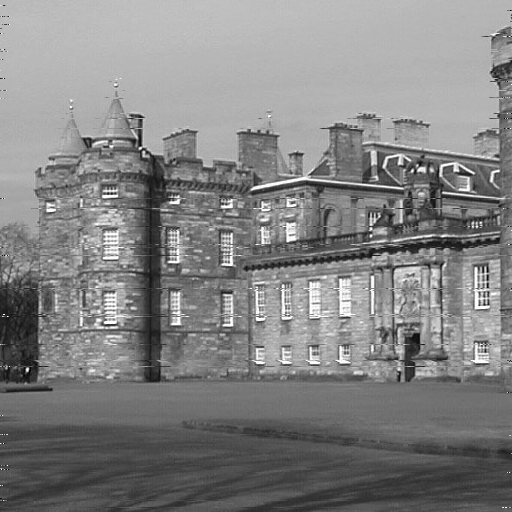
\includegraphics[width=0.95\linewidth]{img/desync1}
  \caption{First input image.}
  \label{fig.6}
\end{minipage}%
\begin{minipage}{.5\textwidth}
  \centering
  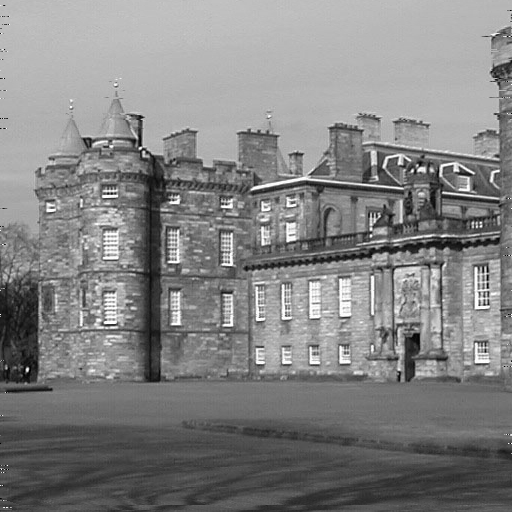
\includegraphics[width=0.95\linewidth]{img/sync1}
  \caption{First image reconstructed.}
  \label{fig.7}
\end{minipage}
\end{figure}

\begin{figure}[h]
\centering
\begin{minipage}{.5\textwidth}
  \centering
  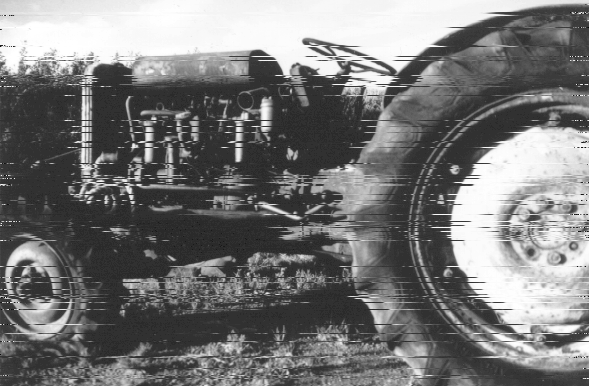
\includegraphics[width=0.95\linewidth]{img/desync2}
  \caption{Second input image.}
  \label{fig.8}
\end{minipage}%
\begin{minipage}{.5\textwidth}
  \centering
  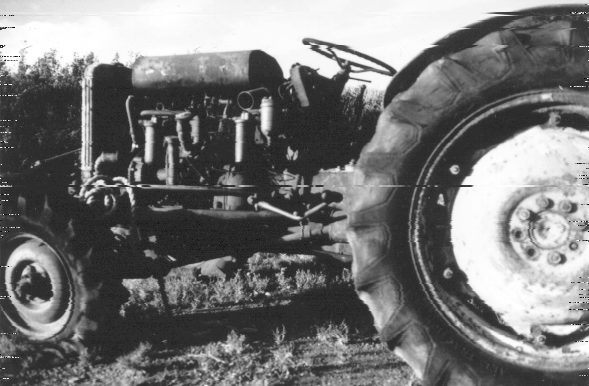
\includegraphics[width=0.95\linewidth]{img/sync2}
  \caption{Second image reconstructed.}
  \label{fig.9}
\end{minipage}
\end{figure}

Figure~\ref{fig.9} is the reconstructed image of fig.~\ref{fig.9}. This was the most problematic image. And the method used, which was very suitable for all the other test images worked less good for this image. The top right hand corner was not adequately reproduced. It also has the ``scratchy'' edges problem of the previous image. However, the reconstructed image is still a good representation of what the actual image would have looked at. 

The last two input images were noticeably better reconstructed with the used algorithm. This is very likely because vertically adjacent lines in these images are more similar to each other, thus leading to more accurate results when using the cross correlation method. 

The third test image still has the problem with loosing information at the edges, but is less serious than in fig.~\ref{fig.7} and~\ref{fig.9}. 

\begin{figure}[h]
\centering
\begin{minipage}{.5\textwidth}
  \centering
  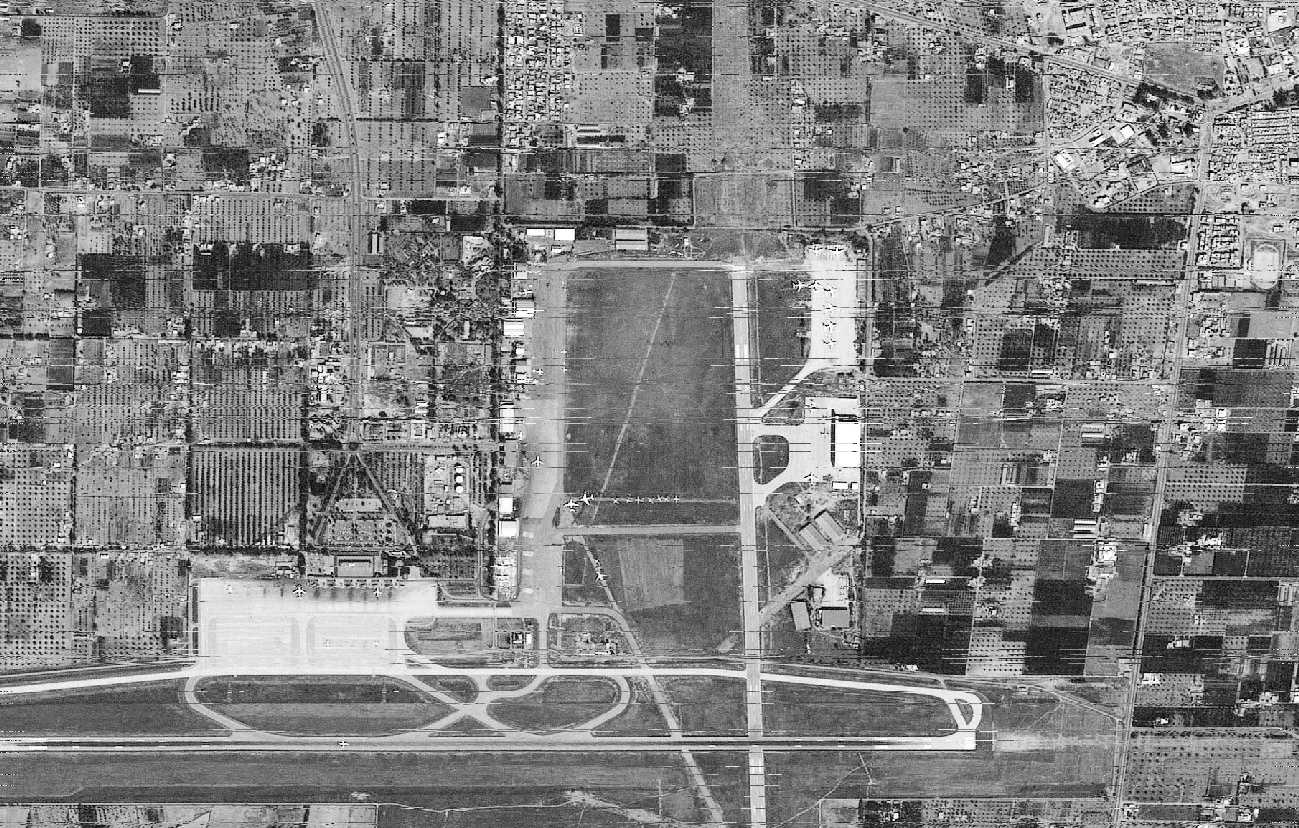
\includegraphics[width=0.95\linewidth]{img/desync3}
  \caption{Third input image.}
  \label{fig.10}
\end{minipage}%
\begin{minipage}{.5\textwidth}
  \centering
  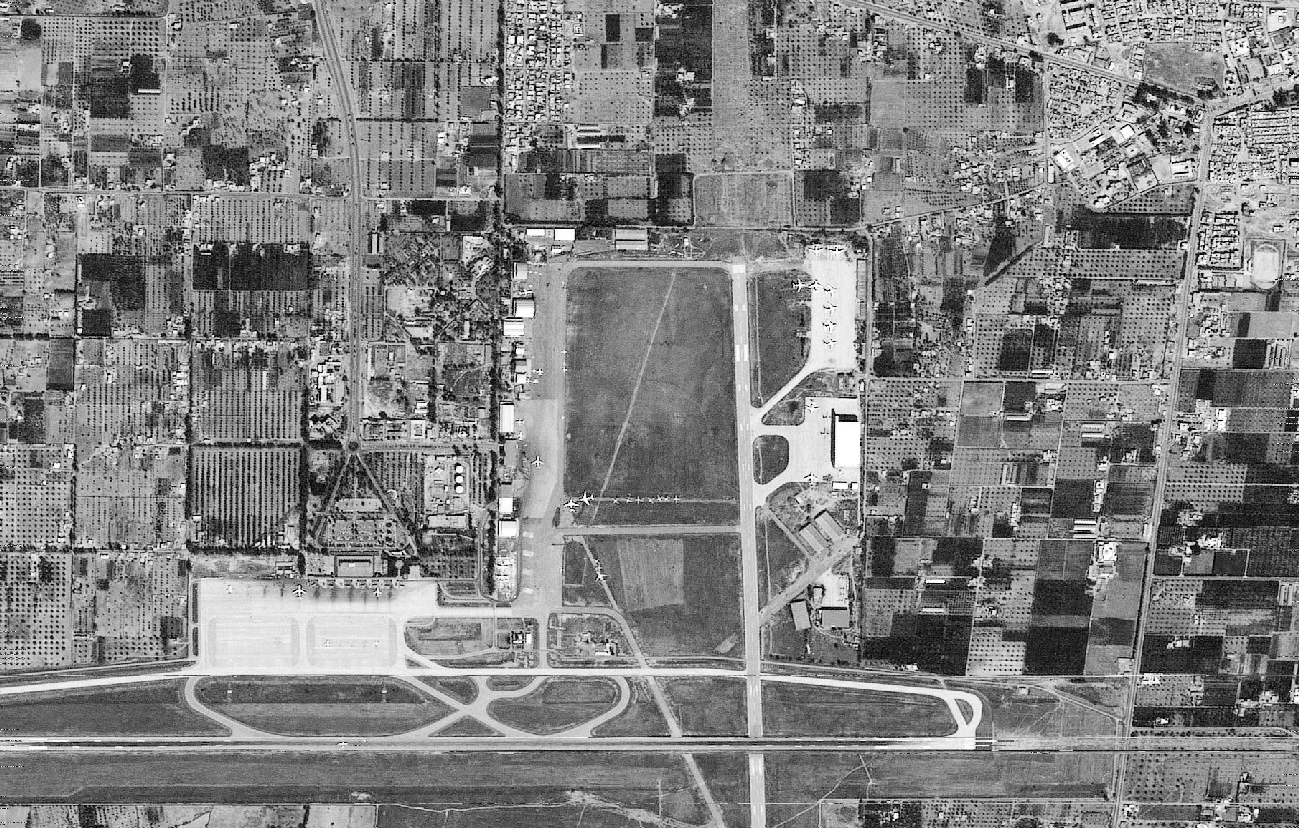
\includegraphics[width=0.95\linewidth]{img/sync3}
  \caption{Third image reconstructed.}
  \label{fig.11}
\end{minipage}
\end{figure}

\begin{figure}[h]
\centering
\begin{minipage}{.5\textwidth}
  \centering
  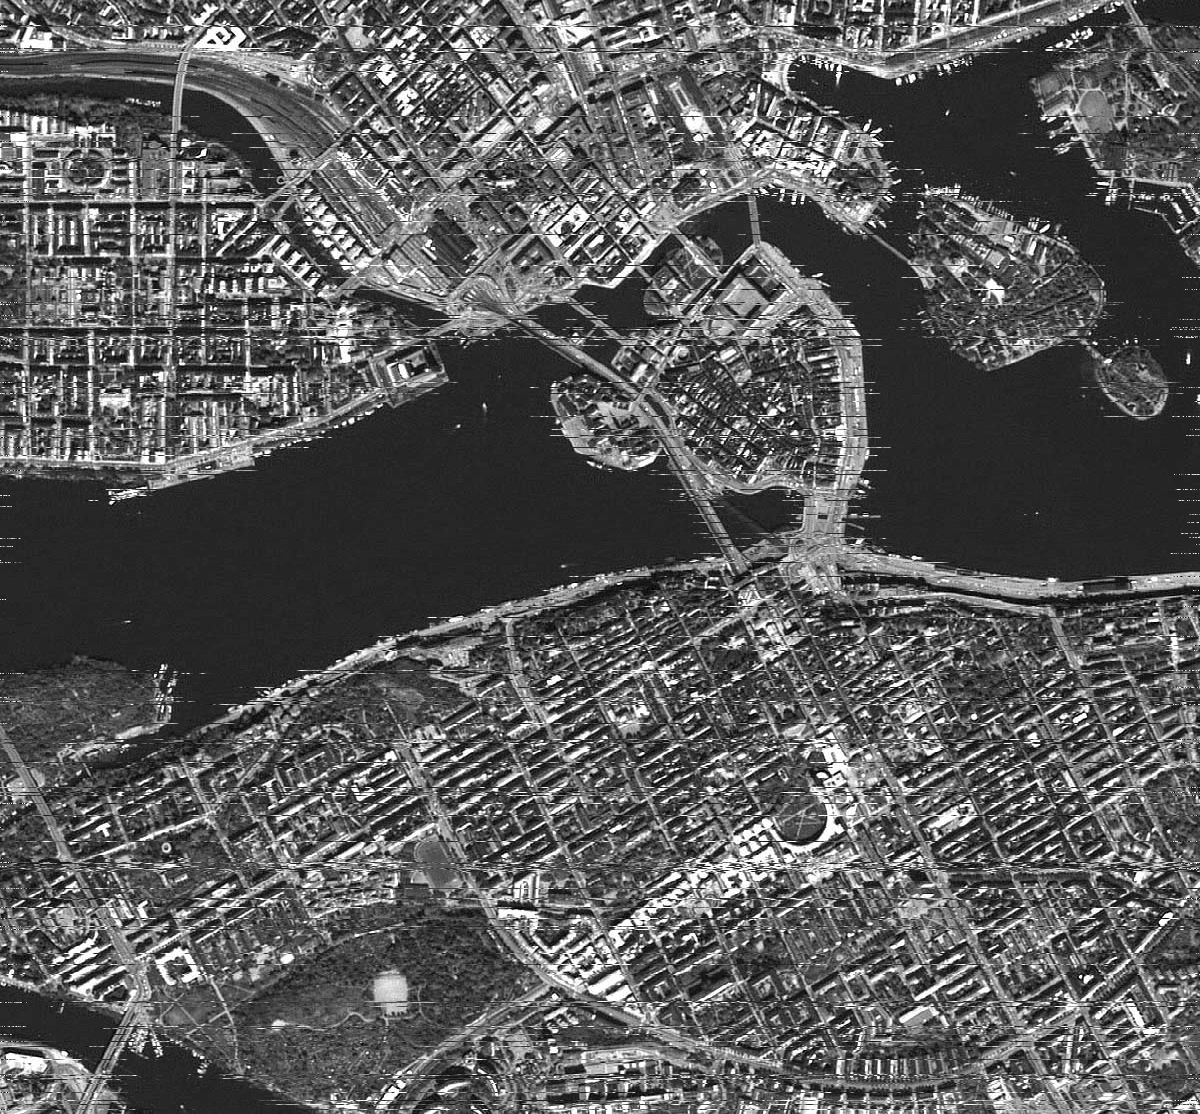
\includegraphics[width=0.8\linewidth]{img/desync4}
  \caption{Fourth input image.}
  \label{fig.12}
\end{minipage}%
\begin{minipage}{.5\textwidth}
  \centering
  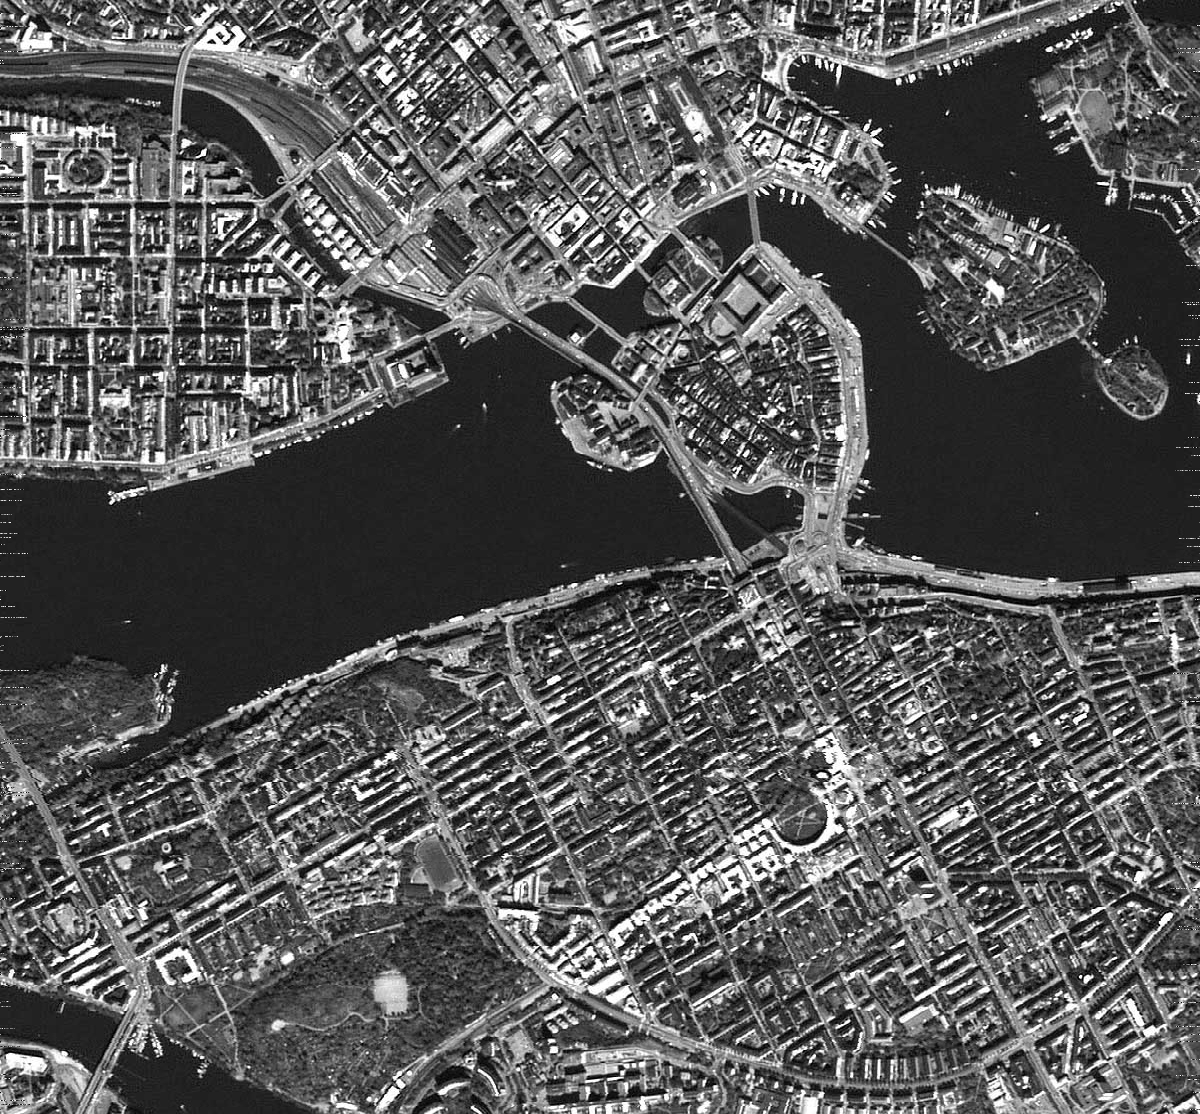
\includegraphics[width=0.8\linewidth]{img/sync4}
  \caption{Fourth image reconstructed.}
  \label{fig.13}
\end{minipage}
\end{figure}

The deviations from a perfect image occur due to the fact that the assumption that vertically adjacent lines are equal at certain times it can be very mistaken. However, in high detail images, this is true more often than not, and hence this type of image has a better reconstruction with the algorithm devised that is based on said assumption. As it was mentioned before, some function could be developed such that the edges have are also reconstructed. 

\newpage

\appendix

\section{Algorithm}

The algorithm used to synchronise the input images is divided into two Python files. The first declares an \texttt{Image} class with the required functions to fix the input image, and the second calls for the user to state what they want image they want to input, and whether or not they want to save the output image. 

\subsection{\texttt{Image.py}}

\begin{lstlisting}[language=numpy]
import numpy as np
import matplotlib.pyplot as plt
from scipy import misc
import os


class Image(object):
    """
     Class to fix a .pgm image with randomly shifted lines.
    :param fileName is the path to a .pgm file
    """

    image = 0.
    cols = 0
    rows = 0

    threshold_top = 0.995 # Maximum value of normalised cross correlation to consider shifting.
    threshold_bottom = 0.8 # Minimum value of normalised cross correlation to consider shifting.

    def __init__(self, fileName):

        self.fileName = str(fileName)
        self.image = misc.imread(self.fileName)
        self.cols = len(self.image)
        self.rows = len(self.image[0])

    def get_xcorrelation(self, line_number):
        """
        :param line_number: int from 1 to rows
        :return: real part of cross correlation between line #line_number and line #line_number-1
        """

        base_line = np.fft.fft(self.image[line_number])
        base_line[:] = (base_line[:]-np.average(base_line))/(np.std(base_line))
        compared_line = np.fft.fft(np.roll(self.image, 1, axis=0)[line_number])
        compared_line[:] = (compared_line[:] - np.average(compared_line)) / (np.std(compared_line))
        xcorrelation = np.fft.ifft(np.multiply(base_line, np.conjugate(compared_line)))

        return xcorrelation.real

    def shift(self):
        """
        Use get_xcorrelation() function to shift the input image into place.
        """

        xcorrelation_max = np.zeros(self.cols)
        shift = np.zeros(self.cols, dtype=int)

        for i in range(1, self.cols):

            xcorrelation = self.get_xcorrelation(i)
            shift[i] = (int)(np.argmax(xcorrelation))
            xcorrelation_max[i] = xcorrelation[shift[i]]

            if (shift[i]!=0) & (shift[i] != shift[i - 1]) & \
                    (xcorrelation_max[i] < self.threshold_top) & (xcorrelation_max[i] > self.threshold_bottom):
                """
                If the shift is non zero, and different from the previous shift (to avoid bulk shifting),
                there will be a shift provided the cross correlation maximum is within an appropriate range.
                """
                self.image[i] = np.roll(self.image[i], -shift[i])

    def clean_up(self):
        """
        Proposed function for cleaning up edges.
        Not used
        """
        cleaned_lines = 0
        xcorrelation_argmax = np.zeros(self.rows)

        for i1 in range(1, self.cols-1):

            xcorrelation_argmax[i1] = np.argmax(self.get_xcorrelation(i1)).astype(int)

        for i1 in range(1, self.cols-1):

            if (xcorrelation_argmax[i1] != 0):

                self.image[i1] = np.roll(self.image, 1, axis=0)[i1]
                cleaned_lines += 1

    def show_image(self):

        plt.imshow(self.image, cmap=plt.cm.gray)
        plt.show(block=False)

    def save_image(self):

        if os.path.isdir("img_out") == False:
            os.mkdir("img_out")

        out_image = str("img_out/" + input("Output image name (just name, not the path) : "))
        misc.imsave(out_image, self.image)
\end{lstlisting}

\subsection{\texttt{FixThem.py}}

\begin{lstlisting}[language=numpy]
from Image import *

fn = str(input("Input image name: "))

while(os.path.isfile(fn) == False):

    fn = str("img_in/" + fn)
    try:
        im = Image(fn)
    except IOError:
        print("File does not exist.")
        fn = str(input("Input image name: "))


im = Image(fn)
im.shift()
#im.clean_up()
im.show_image()

ask_save = str(input("Want to save image? (y/n): "))

if(ask_save == "yes" or ask_save == "y"):

    im.save_image()
\end{lstlisting}

\newpage

\bibliographystyle{unsrt}
\bibliography{report1}

\end{document}
